\begin{tikzpicture}
\tikzset{
    overlay box/.style={fill=white,fill opacity=0.95},
}
\node[overlay,anchor=north west,inner sep=0mm] (base) at (0, 0) {%
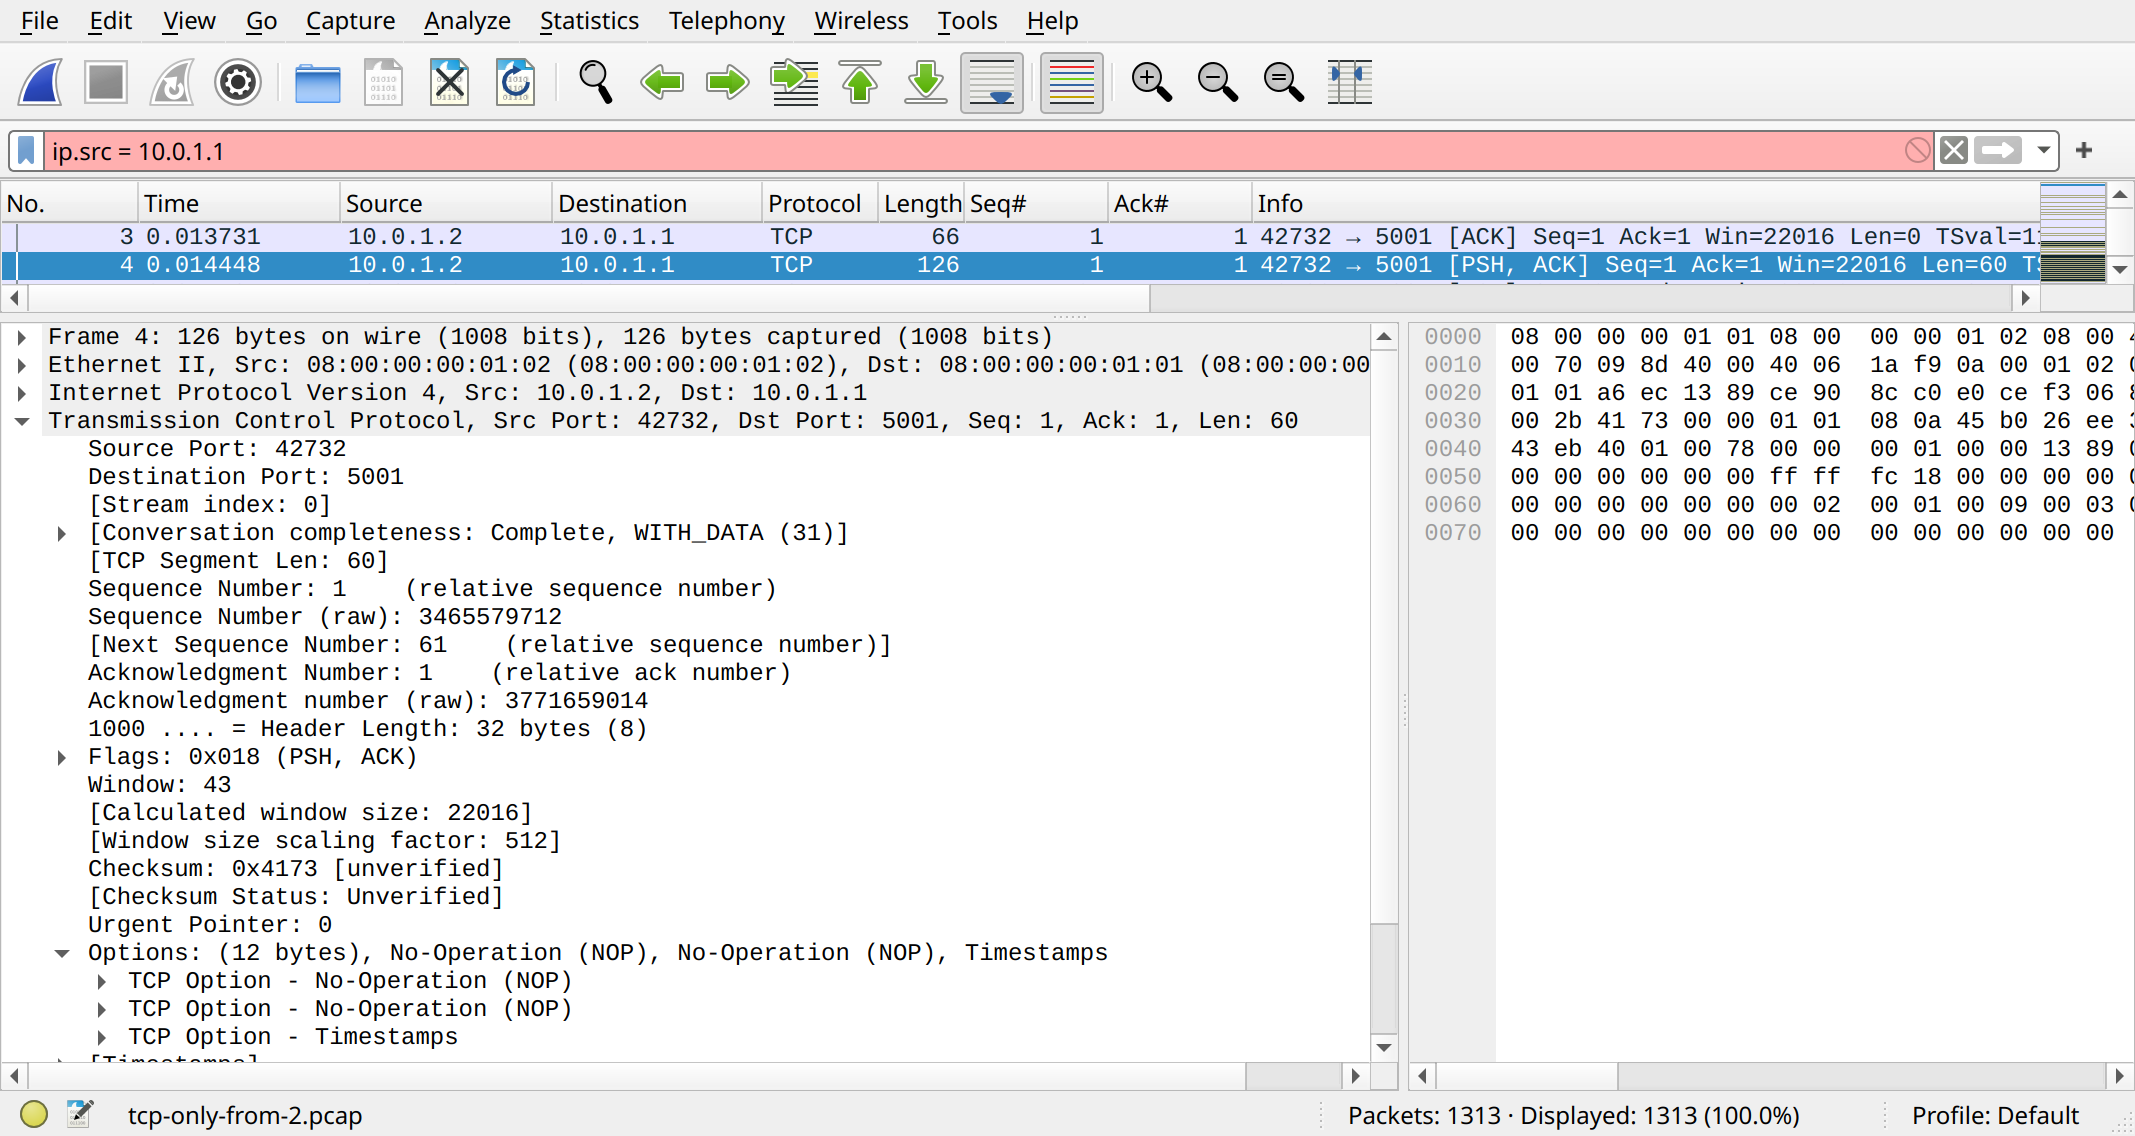
\includegraphics[%
    width=\mypaperwidth,%
    % left bottom right top
    trim={0.5cm 2cm 20cm 10cm},clip,%
]{../reliable/wireshark-tcp-ex2-firstdata}%
};
\path (0, 0) rectangle (14.5, -7); % for bounding box
%\draw[violet,overlay,help lines] (0, 0) grid (14, -8);
%\draw[violet,overlay,help lines,dotted] (0, 0) grid[step=0.2] (14, -8);
%\spy[overlay,rectangle,magnification=1.7,height=7.5cm,width=10cm] on (3, -5) in node at (9, -3.5);
\begin{visibleenv}<2>
    \draw[red,very thick] (0.65, -2.45) rectangle (3.5, -2.75);
    \node[overlay box,text=red,anchor=west,align=left] at (3.5, -2.6) {
        not actually part of header \\
        computed using length from lower layer
    };
\end{visibleenv}
\begin{visibleenv}<3>
    \draw[red,very thick] (0.65, -2.75) rectangle (8.2, -3.25);
    \node[overlay box,text=red,anchor=north west,align=left] at (0.65, -3.25) {
        sequence numbers in header don't start at 0 \\
        wireshark converts to 0-based indices
    };
\end{visibleenv}
\begin{visibleenv}<4>
    \draw[red,very thick] (0.65, -2.75) rectangle (8.2, -3.55);
    \node[overlay box,text=red,anchor=north west,align=left] at (0.65, -3.55) {
        sequence number is \textit{first} byte being sent \\
        need to use segment length to know last byte's number \\
        (= what to ACK if receiving this)
    };
\end{visibleenv}
\begin{visibleenv}<5>
    \draw[red,very thick] (0.65, -3.55) rectangle (7.3, -4);
    \node[overlay box,text=red,anchor=north west,align=left] at (0.65, -4) {
        ack number indicates received start-of-connection stuff \\
        and nothing else (in case server sent something)
    };
\end{visibleenv}
\begin{visibleenv}<6>
    \draw[red,very thick] (0.65, -4.3) rectangle (3.85, -4.6);
    \node[overlay box,text=red,anchor=north west,align=left] at (0.65, -4.6) {
        PSH = no more data right now \\
        ACK = acknowledgment number is valid 
    };
\end{visibleenv}
\begin{visibleenv}<7>
    \draw[red,very thick] (0.65, -4.55) rectangle (5.15, -5.35);
    \node[overlay box,text=red,anchor=south west,align=left] at (0.7, -4.5) {
        window scaling option in use \\
        (scaling factor only sent in connection setup)
    };
\end{visibleenv}
\begin{visibleenv}<8>
    \draw[red,very thick] (0.65, -6.1) rectangle (10.3, -7.2);
    \node[overlay box,text=red,anchor=south west,align=left] at (0.7, -6.0) {
        no-operation options used to make TCP header size multiple of 4
    };
\end{visibleenv}
\end{tikzpicture}